%\section{Defining the neutrino floor/fog by discovery potential}
\section{The neutrino fog}
\label{sec:neutrinofloor}

As direct dark matter searches accumulate ever larger exposures in pursuit of testing smaller interaction cross sections, the expected background from the coherent elastic neutrino-nucleus scattering (CE$\nu$NS) of astrophysical neutrinos increases. For dark matter masses $\gtrsim10$~GeV/$c^2$, the relevant neutrino fluxes are those from $^8$B solar neutrinos, atmospheric neutrinos, and the diffuse supernova neutrino background (DSNB). The CE$\nu$NS event rate from each of these is subject to a systematic uncertainty which manifests from the uncertainty on the flux of each neutrino species. In addition, the nuclear recoil energy spectra of these events closely resembles that of the sought after dark matter signal -- this is the case for a spin-independent (SI) dark matter interaction as well as for other couplings/interactions. An example is given in Fig.~\ref{fig:coherent_solarnu_rates}, which shows the SI nuclear recoil rate of a couple of WIMP masses on xenon and argon alongside those of the dominant neutrino backgrounds. 

The effect of these backgrounds -- particularly because of their associated systematic uncertainties and spectral shapes --  will be to reduce the dark matter sensitivity achievable as the experimental exposure grows. This fact led to the creation of the colloquially known ``neutrino floor": a boundary in the cross section versus dark matter matter mass plane below which a dark matter discovery becomes extremely challenging without further constraints on the neutrino backgrounds. The precise location of this boundary has evolved over the last decade~\cite{Billard:2013qya,Gelmini:2018ogy,OHare:2020lva,OHare:2021utq}, however more recent studies~\cite{OHare:2020lva,OHare:2021utq} have emphasized a crucial point: that astrophysical neutrino backgrounds do not impose a hard limit on physics reach; rather, the effect is more gradual than a single boundary depicts. To reinforce this concept within the community, the term ``neutrino fog" has instead been used to describe the region of dark matter cross sections where neutrino backgrounds begin to inhibit the progress of direct detection searches.


\subsection*{Defining the neutrino fog}

We choose to adopt the methodology of O'Hare~\cite{OHare:2021utq} in defining the neutrino fog region, with astrophysicsl parameters updated to match the recommendation in Ref.~\cite{recommendation_dark_matter}. Specifically, the quantity of interest is the index $n$, defined as the gradient of a hypothetical experiment's median cross section for $3\sigma$ discovery with respect to the exposure:

\begin{equation}
    n = -\bigg( \frac{d \log{\sigma}}{d \log{MT}} \bigg)^{-1}
\end{equation}

This index quantifies the diminishing return-on-investment in increasing exposure when limited by neutrinos. Specifically, if an experiment has achieved some cross-section sensitivity, further reducing the sensitivity by a factor of $x$ requires increasing the exposure by at least $x^n$. E.g., at $n=2$, reducing the cross section reach by a further factor of 10 requires increasing the exposure by a factor of at least 100. 

In order to illustrate the ever-diminishing returns due to the neutrino fog, in Figure~\ref{fig:limitplot_SI}, we plot contours of the index. In order to simplify the contours, the maximum index is projected down.  If the neutrino fog must be represented by a single line, we choose $n=2$, as this marks the transition from statistically- to systematically-limited. Figure~\ref{fig:exposure_at_floor_SI} illustrates the exposure necessary for a handful of targets for spin-independent couplings. A critical feature of the neutrino fog is that it will move to lower cross section if uncertainties in the neutrino fluxes are reduced, opening up new space for continuing searches. 

\begin{figure}
    \centering
    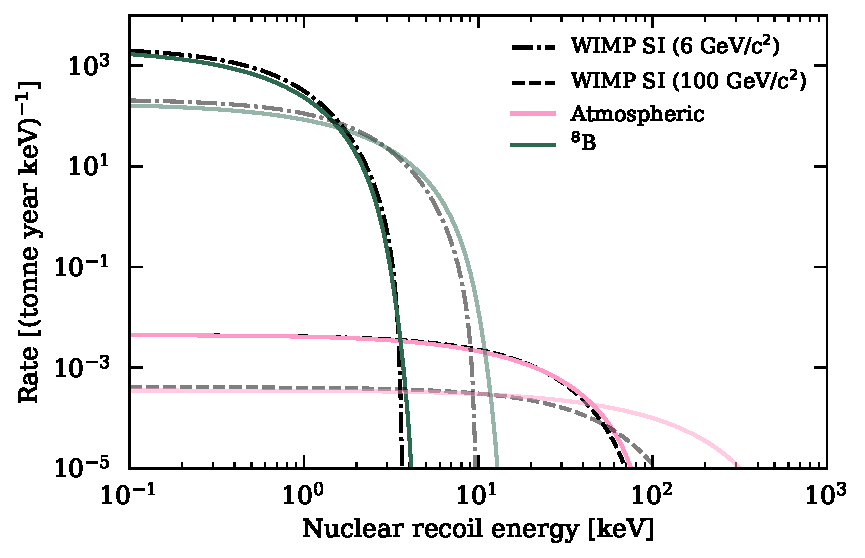
\includegraphics[width=0.75\textwidth]{figures/nu_rates_coherent_combined.pdf}
    \caption{Spectrum of solar-neutrino nuclear recoils scattering on Xe (darker color) and Ar (lighter color). The recoil spectrum for a 6 GeV/$c^2$ (dashed line) and a 100 GeV/$c^2$ (dotted-dashed line) are also given for reference.}
    \label{fig:coherent_solarnu_rates}
\end{figure}

\begin{figure}
    \centering
    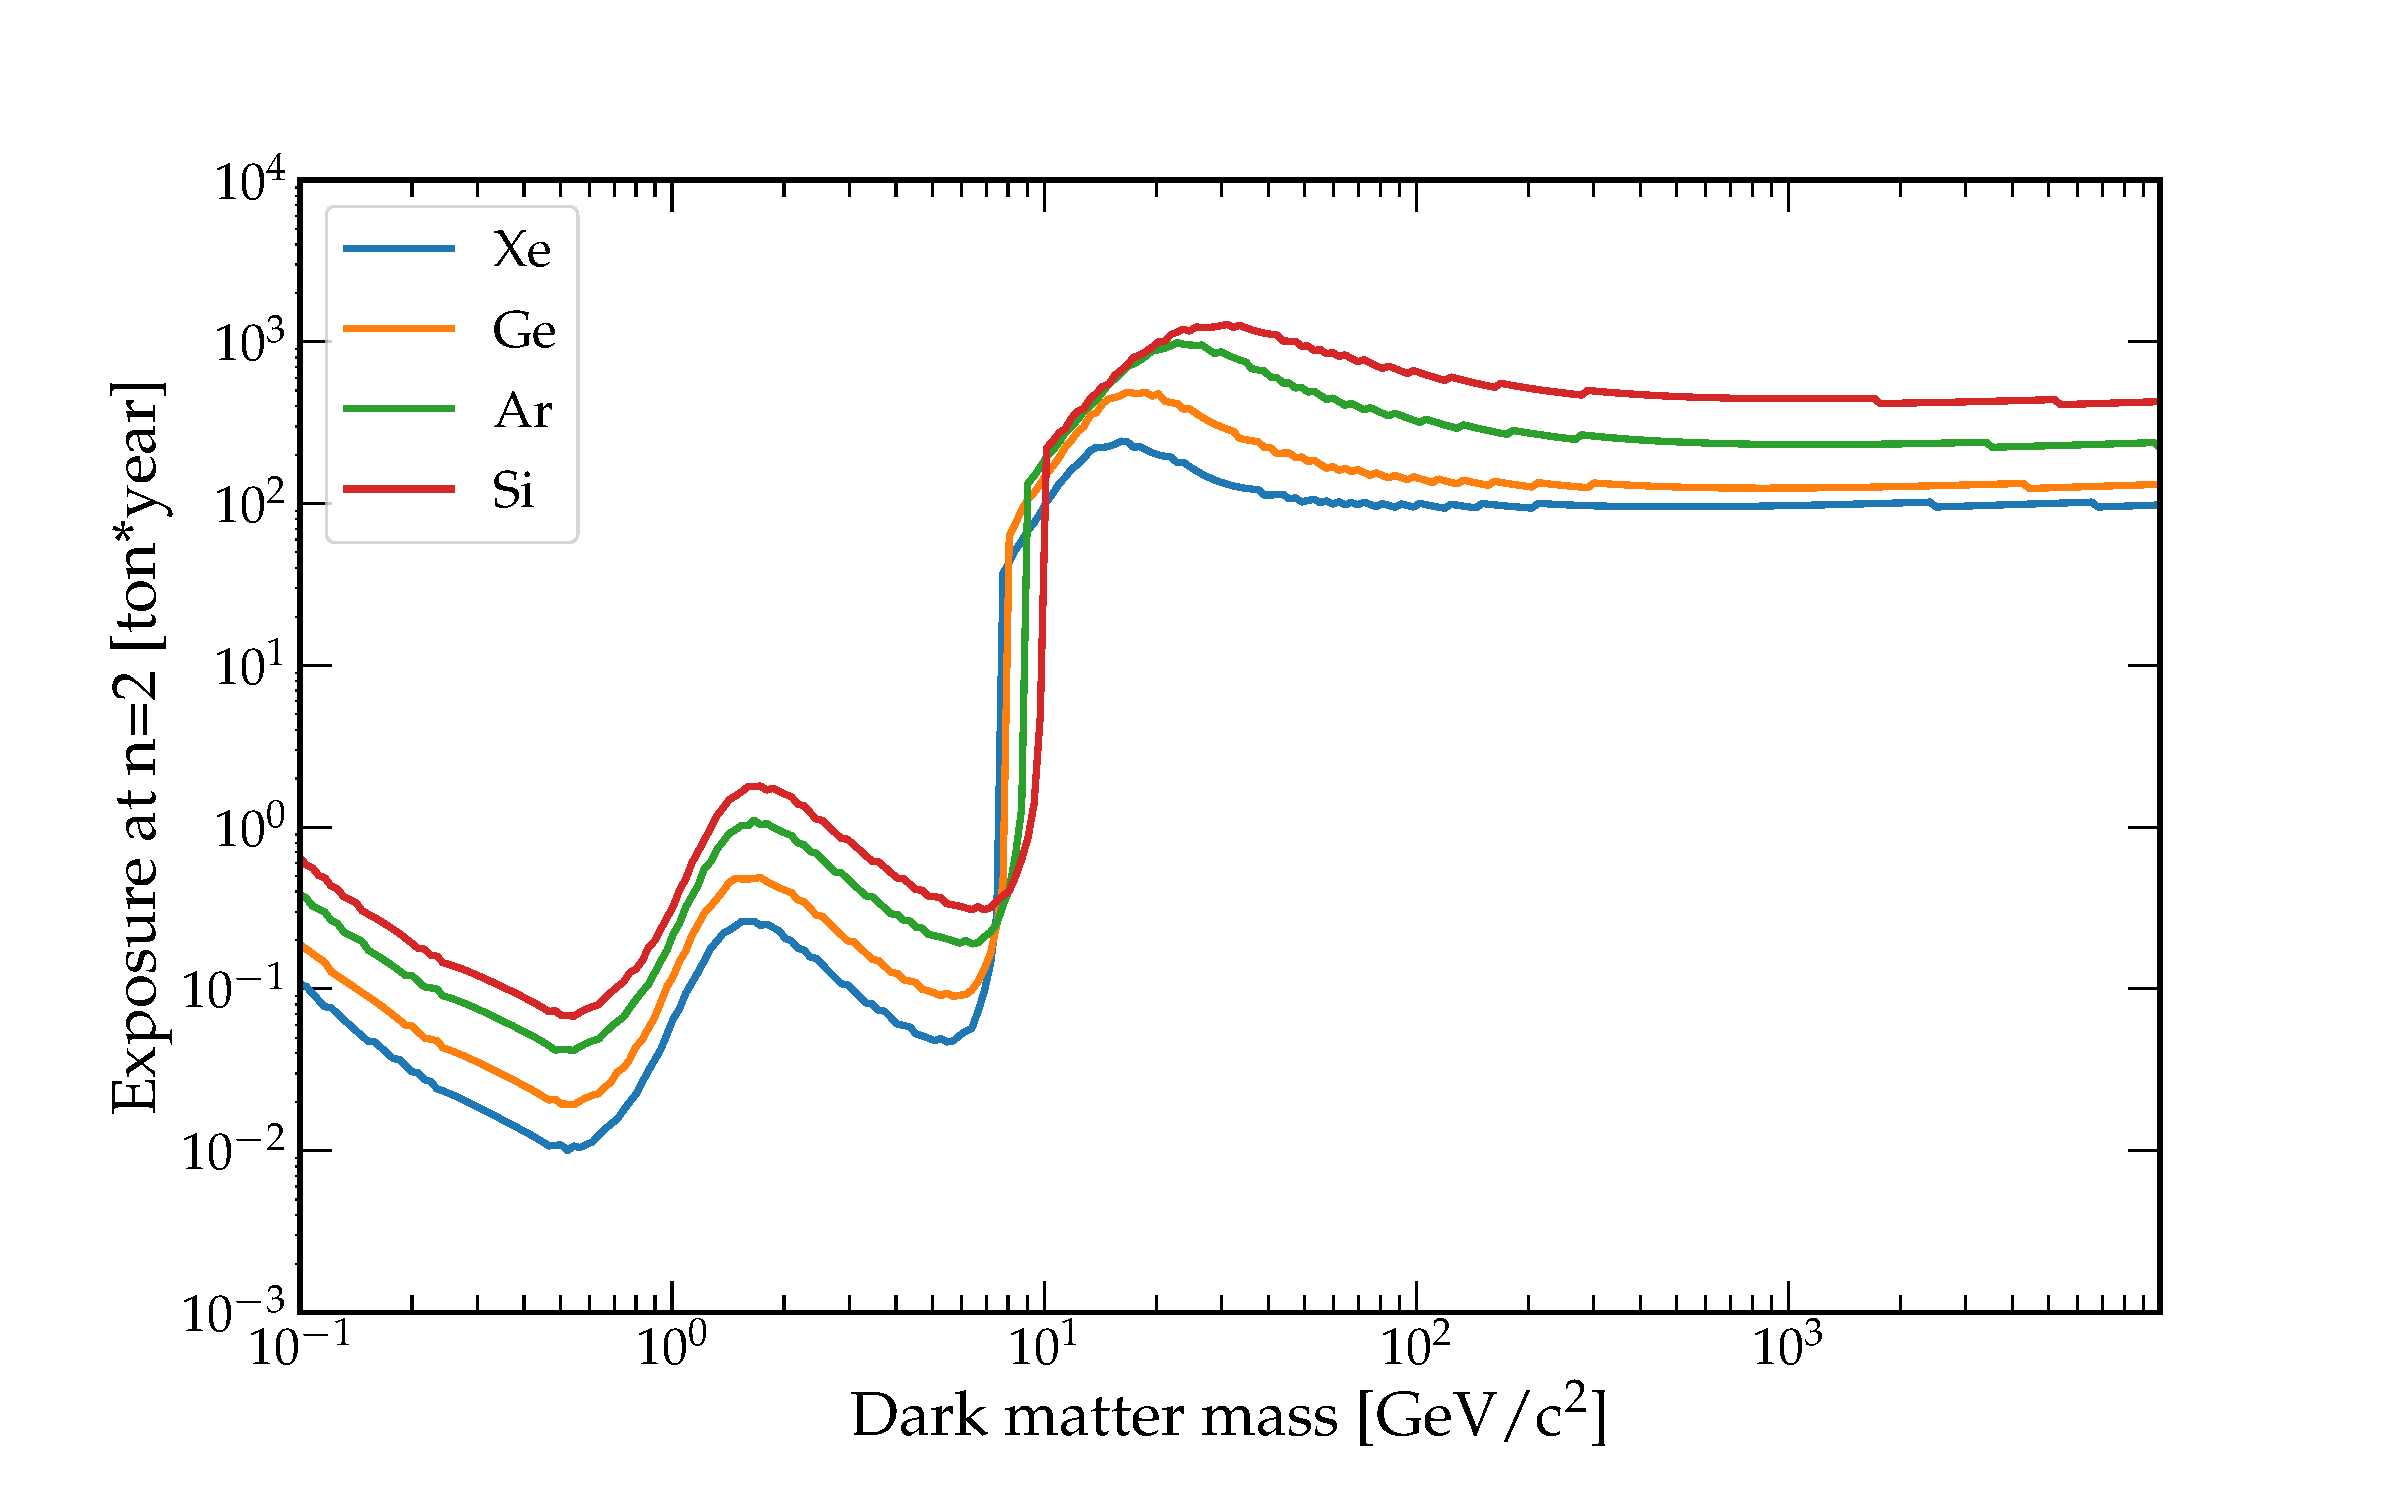
\includegraphics[width=0.8\textwidth]{figures/exposure_at_floor_SI.pdf}
    \caption{Exposure in ton-years required to reach the $n=2$ (systematic-limited) spin-independent neutrino fog level as a function of dark matter mass for various targets. 
    \label{fig:exposure_at_floor_SI}}
\end{figure}